% IEEE journal-style FINAL report (Semesters 1 + 2)
% Intelligent Multi-Disease Risk Prediction System

\documentclass[journal]{IEEEtran}

\usepackage{graphicx}
\usepackage{booktabs}
\usepackage{multirow}
\usepackage{amsmath}
\usepackage{amsfonts}
\usepackage{cite}
\usepackage[hidelinks]{hyperref}

\title{Intelligent Multi-Disease Risk Prediction System with Explainability}

\author{Avula~Lakshmi~Narasimha~Reddy~(S20230010030),~Rayapu~Nishanth~(S20230010202)%
\thanks{Bachelor Thesis Project (BTP) 2025--2026, B.Tech (CSE), Indian Institute of Information Technology, Sri City (IIIT Sri City), India.}%
\thanks{Guide: Dr.~R.~Selvi (IIIT Sri City).}%
}

\markboth{BTP Final Report (Semesters 1 \& 2), 2025--2026}{BTP Final Report}

\begin{document}
\maketitle

\begin{center}
\textit{Final Report --- Bachelor Thesis Project 2025--2026}\\[2pt]
\textit{Guided by Dr.~R.~Selvi (IIIT Sri City)}
\end{center}

\begin{abstract}
Multi-morbidity --- the co-occurrence of chronic conditions in one patient --- is increasingly the norm rather than the exception, yet the majority of public datasets and prototype tools remain organized around a single disease. This report documents the complete two-semester development of an intelligent multi-disease risk prediction platform that fuses four heterogeneous clinical cohorts (Diabetes, Heart Disease, Liver Disease, Kidney Disease) into one unified 24-feature schema and answers a harder question: does data measured for one disease carry predictive signal for another? Semester~1 built the data foundation --- dataset selection and harmonization, a unified clinical schema, explicit handling of \emph{structural missingness} through two competing encodings (masked and sentinel), four classical baselines (Logistic Regression, Random Forest, XGBoost, LightGBM), and a multi-output FT-Transformer --- and validated a formal hypothesis about which encoding suits which model family. Semester~2 converted the research prototype into a production-grade system: a shared inference engine driving a Streamlit application, a FastAPI service, and a generated six-page patient PDF report; exact per-patient TreeSHAP explanations; a clinical NLP layer extracting lifestyle factors from free text; a provider-agnostic LLM explanation and chat layer with safety guardrails; and a novel \emph{cross-disease signal analysis} --- per-patient attribution by feature family, panel ablation, and marker-coverage gating --- that makes the fusion thesis measurable. Final deployed test AUC-ROC: Diabetes~0.938, Heart~0.801, Liver~0.999, Kidney~0.971. A dataset-level interrelation stress test confirms cross-disease transfer in 3 of 5 scenario pairs; negative results are reported honestly rather than suppressed.
\end{abstract}

\begin{IEEEkeywords}
Multi-disease prediction, dataset fusion, structural missingness, sentinel encoding, masked encoding, XGBoost, LightGBM, FT-Transformer, SMOTE, SHAP, cross-disease attribution, ablation study, FastAPI, Streamlit, clinical NLP, large language models.
\end{IEEEkeywords}

% ══════════════════════════════════════════════════════════════════
\section{Introduction}
Chronic diseases rarely occur in isolation. Diabetes drives chronic kidney disease and cardiovascular disease; liver dysfunction alters lipid metabolism; hypertension is simultaneously a cardiac risk factor and a cause of renal decline. Clinical risk assessment is therefore inherently multi-disease --- yet the tooling landscape does not reflect this. Public datasets are collected per disease, each measuring a different biomarker panel; published baselines address one condition at a time; and the few existing multi-disease apps simply place independent models side by side without any shared representation, so a patient's diabetes labs can never inform their kidney estimate.

This project began from two questions:
\begin{enumerate}
    \item \textbf{Fusion:} can four heterogeneous disease cohorts, each measuring a different biomarker panel, be unified into one feature schema without corrupting the per-disease signal?
    \item \textbf{Transfer:} once fused, does information associated with one disease genuinely contribute to risk estimation for another --- and can we \emph{measure} that contribution rather than assume it?
\end{enumerate}

Over two semesters we built a complete answer, and this report documents the whole arc. \textbf{Semester~1} (Sections~II--X) was the research phase: dataset selection, schema engineering, a formal treatment of the missingness problem that fusion inevitably creates, and a model benchmark spanning a linear baseline through gradient-boosted trees to a deep transformer. \textbf{Semester~2} (Sections~XI--XVIII) was the engineering phase: turning the chosen models into a consistent, explainable, deliverable system --- one shared inference engine behind a web application, a REST API, and an automated patient report --- plus the analysis machinery that makes the transfer question answerable with numbers.

The contributions, in summary:
\begin{itemize}
    \item A unified 24-feature clinical schema integrating four cohorts ($\approx$191{,}000 rows after deduplication), with explicit encodings for \emph{structural missingness} and a validated hypothesis about which encoding suits which model family.
    \item A benchmark of five model families under two missingness encodings, with full metrics and a principled deployment decision (XGBoost) that weighs more than raw AUC.
    \item A production system --- Streamlit app, FastAPI service, six-page PDF report --- served by one shared inference engine so that all surfaces return byte-identical predictions.
    \item An explanation stack spanning exact TreeSHAP attributions, patient-facing NLP context notes, and a guardrailed LLM guidance layer with a rule-based fallback.
    \item A cross-disease analysis suite (attribution, ablation, coverage gating, dataset-level stress test) that quantifies the transfer claim and honestly flags its limits.
\end{itemize}

% ══════════════════════════════════════════════════════════════════
\section{Background and Design Context}
\subsection{Why tabular machine learning, and which family?}
Clinical biomarker data is tabular: a fixed set of numeric features per patient. For tabular data, gradient-boosted decision trees (GBDTs) remain the dominant approach --- they consistently match or beat deep networks on medium-sized tabular benchmarks while being far cheaper to train and serve. We therefore treat GBDTs as the deployment candidate and evaluate four model families that span the classic capacity spectrum: a linear model (Logistic Regression), a bagged tree ensemble (Random Forest), and two boosting implementations (XGBoost and LightGBM). A fifth, deep model (FT-Transformer) tests whether attention-based feature interaction modeling can beat the classical ceiling. Each model is described in detail where it is introduced (Section~VII).

\subsection{Missing data is not a nuisance --- it is the problem}
Standard missing-data theory distinguishes MCAR (missing completely at random), MAR (at random given observed values), and MNAR (not at random --- absence depends on the unobserved value itself). Our fusion problem creates a fourth pattern we call \emph{structural missingness}: a feature is absent for an entire cohort because that disease panel simply never measures it --- liver enzymes do not exist in a cardiac cohort's schema. This is neither random nor recoverable by imputation: an imputer that ``fills in'' a liver enzyme from cardiovascular features would fabricate a measurement that was never taken, teaching the model correlations that do not exist in any real patient. Missingness must therefore be represented explicitly, which motivates the dual-encoding design of Section~V.

\subsection{Explainability requirement}
A risk score that cannot say \emph{why} is not clinically usable. We require attributions that are (i)~exact rather than approximated, (ii)~per-patient rather than only global, and (iii)~renderable for non-technical readers. SHAP (SHapley Additive exPlanations)~\cite{lundberg2017shap} assigns each feature a signed contribution to a prediction; its tree-specific variant, TreeSHAP~\cite{lundberg2020treeshap}, computes \emph{exact} Shapley values for tree ensembles in polynomial time instead of sampling approximations. This requirement later constrains model selection (Section~X): the deployed model must support faithful per-instance attribution.

% ══════════════════════════════════════════════════════════════════
\section{Datasets}
\subsection{Selection criteria and cohorts}
We required publicly available tabular cohorts with (i)~clinically meaningful biomarker measurements (not derived survey scores alone), (ii)~sufficient sample size for stable training, and (iii)~a clear binary disease label. Four cohorts met the bar (Table~\ref{tab:datasets}).

\begin{table}[t]
\centering
\caption{Source Cohorts}
\label{tab:datasets}
\small
\begin{tabular}{lccc}
\toprule
\textbf{Cohort} & \textbf{Samples} & \textbf{Share} & \textbf{Label balance} \\
\midrule
Diabetes  & 100{,}000 & 52.3\% & diabetic / non-diabetic \\
Heart     & 70{,}000  & 36.6\% & disease / no disease \\
Liver     & 30{,}691  & 10.1\% & liver disease / none \\
Kidney    & 1{,}659$\to$2{,}032 (SMOTE) & 1.1\% & CKD / non-CKD \\
\midrule
\textbf{Unified (deduped)} & \textbf{$\approx$191{,}363} & 100\% & 4 target columns \\
\bottomrule
\end{tabular}
\end{table}

The imbalance across cohorts is itself a design constraint: diabetes and heart dominate, while kidney contributes barely 1\% of rows --- one reason its model behaves differently under missing panels (Section~XIII).

\subsection{Deviation: breast cancer replaced by kidney disease}
The original proposal listed breast cancer among the target diseases. We replaced it, and this was a deliberate fusion-driven decision: the Wisconsin-style cohorts measure tumor-cell morphology (radius, texture, concavity of nuclei) --- features with zero overlap against laboratory biomarkers. A model over such features could coexist in a pipeline but could never participate in \emph{heterogeneous clinical fusion}, the project's core contribution. Kidney disease, by contrast, is the proposal's own ``extended coverage'' option, shares features with other cohorts (blood pressure, hemoglobin, BMI), and enables the clinically real cardiorenal and diabetic-nephropathy narratives the transfer question needs.

\subsection{One label per row}
A property of fusion that shapes every methodological choice: each unified row originates from exactly one source cohort, so only \emph{its own} disease label is observed. A diabetes-cohort row has no heart label --- that label is not negative, it is \emph{unobserved}. Treating unobserved labels as negatives would inject hundreds of thousands of false counterexamples; instead we train each disease head only on rows where its label exists (Section~VII), and for the deep model we apply a masked loss that simply skips unobserved heads (Section~VII-E).

% ══════════════════════════════════════════════════════════════════
\section{Unified Clinical Schema}
Fusion requires a shared feature space. We designed a 24-feature schema spanning five clinical panels (Fig.~\ref{fig:schema}): demographics (age, gender, BMI); cardiovascular (systolic and diastolic blood pressure, total cholesterol, HDL, LDL, triglycerides); diabetes (fasting glucose, HbA1c); liver (ALT, AST, ALP, albumin, total protein, total and direct bilirubin, A/G ratio); and kidney (serum creatinine, BUN, GFR, urine protein, hemoglobin).

\begin{figure}[t]
\centering
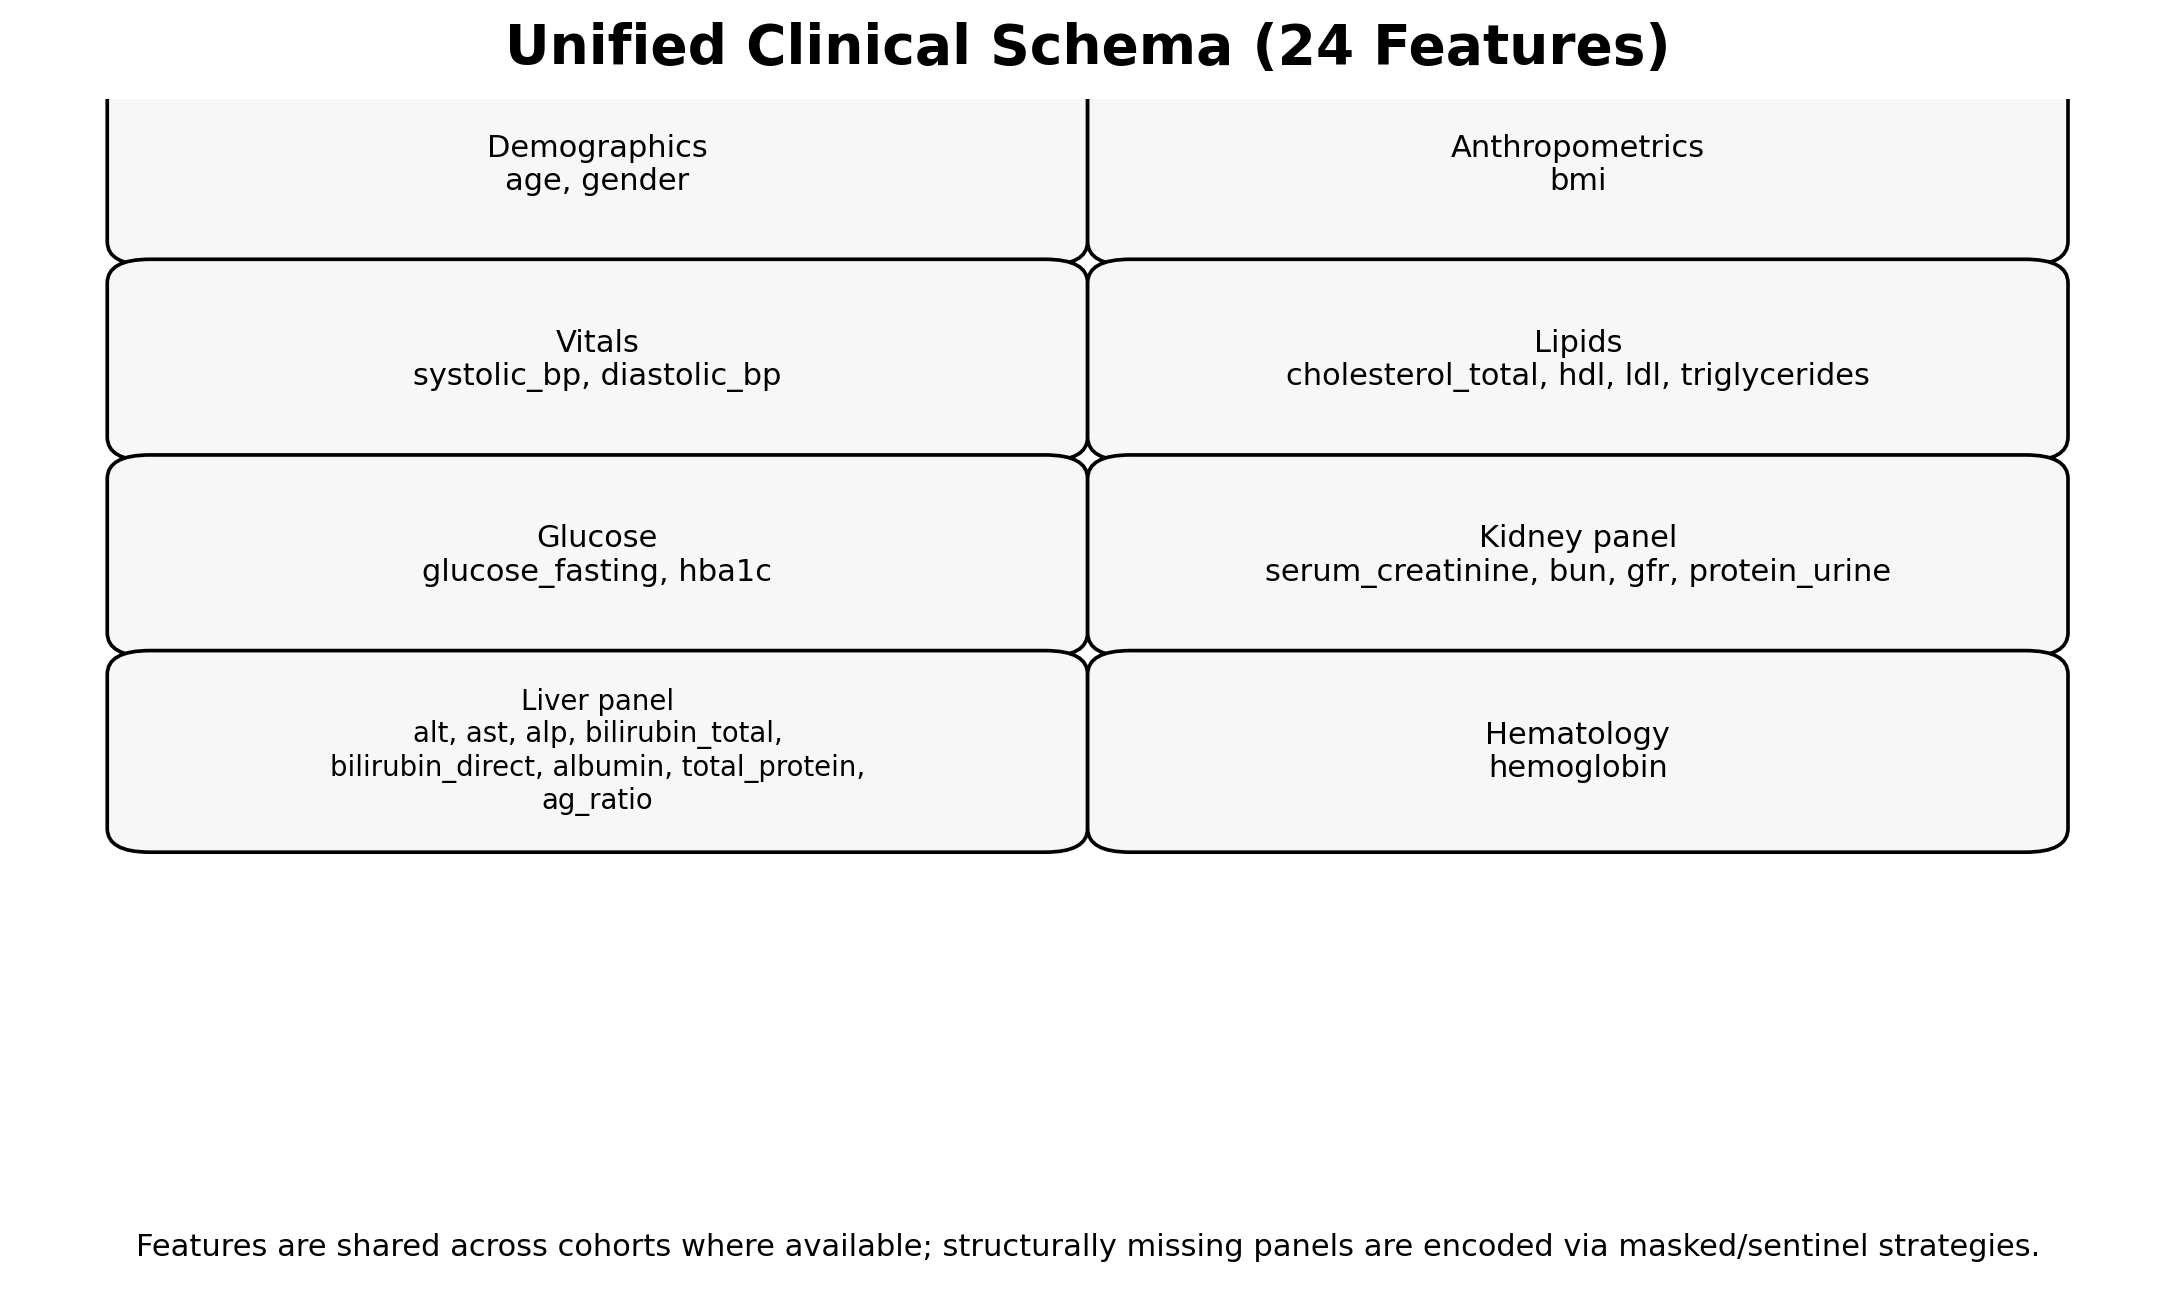
\includegraphics[width=\linewidth]{report_figures/unified_schema_24_features.png}
\caption{Unified clinical schema: 24 features grouped by clinical panel.}
\label{fig:schema}
\end{figure}

Three schema decisions illustrate the engineering behind what is otherwise ``just a column list'':
\begin{enumerate}
    \item \textbf{Derived features:} BMI is a strong shared risk factor but absent from the heart cohort's export --- we derived it from height and weight where available rather than dropping it or marking it unobserved for 70{,}000 rows.
    \item \textbf{Unit and scale harmonization:} categorical encodings had to be reconciled --- e.g., the heart cohort stores cholesterol as an ordinal bucket (normal/above/well-above) while other cohorts store mg/dL; we mapped buckets to approximate numeric midpoints so a single numeric feature could represent the quantity, accepting the quantization error as a documented limitation.
    \item \textbf{Keep the disease-specific features:} features measured by only one cohort (e.g., bilirubin for liver, urine protein for kidney) were retained, not dropped --- they are precisely the ``own panels'' that let each disease model specialize, and their structured absence is handled by the encoding layer next.
\end{enumerate}

% ══════════════════════════════════════════════════════════════════
\section{Structural Missingness: Two Encodings}
\subsection{Why conventional imputation is unsafe here}
When a feature is missing for random reasons, imputation is reasonable. Structural missingness is different: the liver enzyme is not an unlucky blank in a heart record --- it was never in the heart panel at all. Imputing it from shared features (age, BMI, lipids) produces a hallucinated measurement; worse, the imputed value is a deterministic function of the cross-disease features, so a model can no longer distinguish ``measured normal'' from ``never measured.'' We therefore encode the fact of missingness itself.

\subsection{Masked representation: value + availability indicator}
For the deep model, every numeric feature $x_j$ is paired with a binary availability flag $m_j\in\{0,1\}$:
\begin{equation}
\tilde{x}_j = \begin{bmatrix}x_j \\ m_j\end{bmatrix},\qquad
m_j = \begin{cases}1 & \text{observed}\\0 & \text{structurally absent}\end{cases}
\end{equation}
Absent values are filled with a conservative statistic (cohort median) so the value channel stays finite, but the mask tells the network to discount it. This is the richer representation --- it keeps ``what the value would be'' and ``whether it exists'' in separate channels, which is exactly what an attention mechanism can exploit.

\subsection{Sentinel representation: a value outside reality}
For tree-based models we chose a different encoding: missing numerics become a sentinel constant of $-999$. The reasoning is specific to how decision trees work. All real features are standardized (zero mean, unit variance over observed values only), so genuine measurements live near $[-4,4]$, while $-999$ sits astronomically far away. Any tree split of the form ``$x_j < -500$?'' cleanly separates ``absent'' from ``observed'' in a single node --- the tree \emph{learns} missingness as a feature without any extra columns, keeping the deployed feature count at 24.

\subsection{The scaling subtlety}
Standardization must not destroy the encoding. For the sentinel version we fit the scaler on non-sentinel values only and apply it to non-sentinel values, leaving $-999$ untouched; a na\"{\i}ve scaler would drag the sentinel toward the mean and mix ``absent'' with ``extreme value.'' For the masked version, only value channels are scaled; mask columns remain binary. The full pipeline is summarized in Fig.~\ref{fig:missingness}.

\begin{figure}[t]
\centering
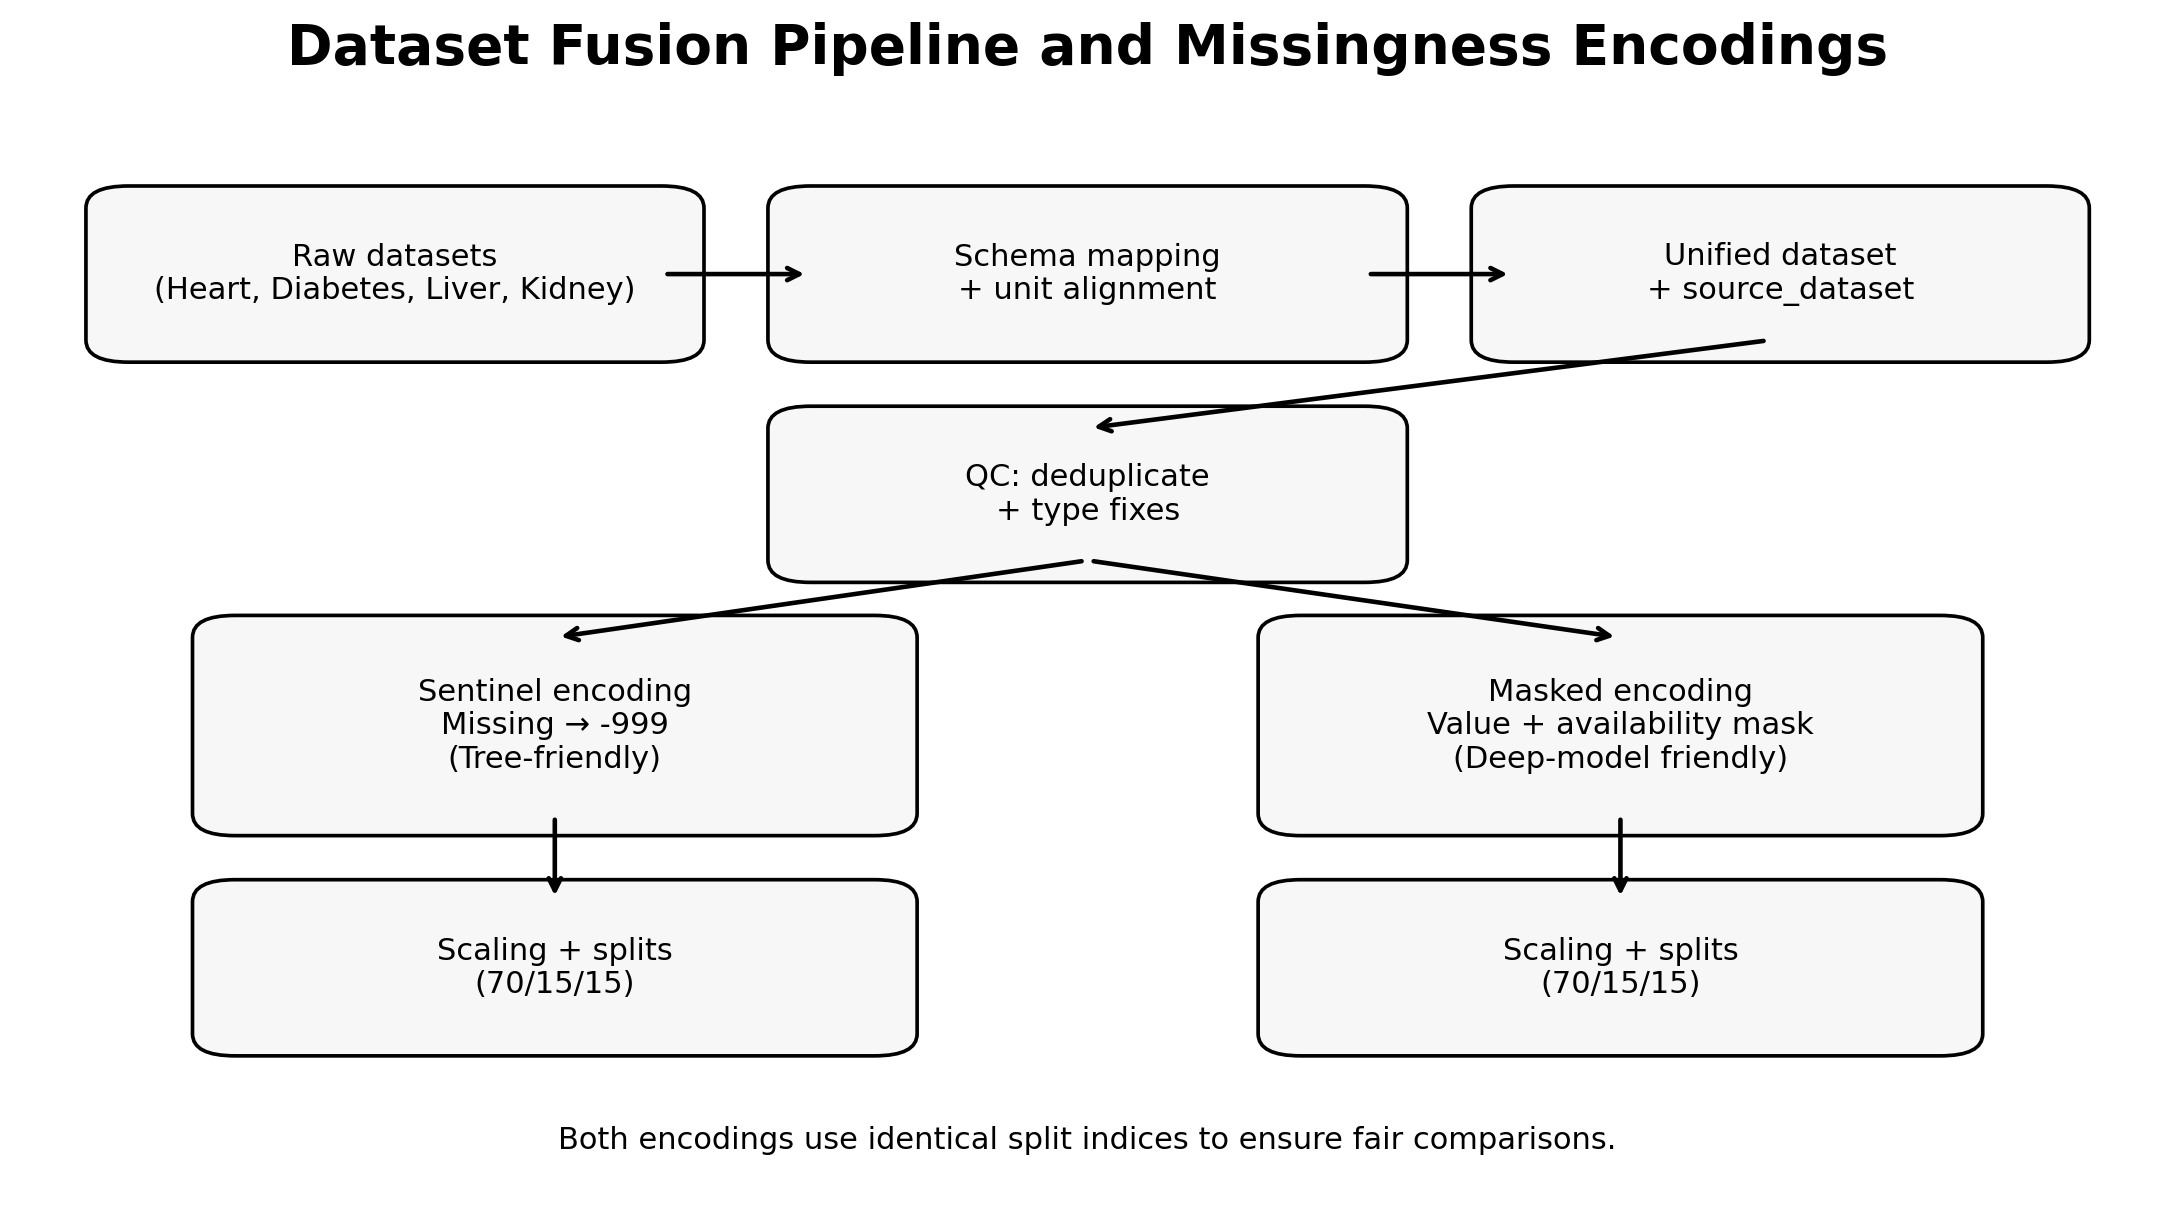
\includegraphics[width=\linewidth]{report_figures/data_pipeline_masked_sentinel.png}
\caption{Fusion and missingness pipeline: per-cohort harmonization into the 24-feature schema, then two parallel encodings --- masked (value+mask) for the transformer and sentinel ($-999$) for tree models.}
\label{fig:missingness}
\end{figure}

\subsection{The Week-4 hypothesis}
Before benchmarking we wrote down a falsifiable prediction: \emph{sentinel encoding is sufficient for tree models (they can split around it), while explicit masks provide richer signal for attention-based models.} Section~IX shows how this hypothesis was tested and confirmed --- and where it failed in an instructive way.

% ══════════════════════════════════════════════════════════════════
\section{Preprocessing Protocol}
\subsection{Deduplication}
Exact duplicate records were removed cohort-wide: $\approx$11{,}360 rows, concentrated in the liver dataset (a known artifact of that cohort's publication format). Deduplication matters because duplicate rows that straddle the train/test boundary would inflate metrics --- the model would effectively memorize rather than generalize.

\subsection{Class imbalance: SMOTE for the kidney cohort}
The kidney cohort had 1{,}659 usable rows with a minority positive class. We applied SMOTE~\cite{chawla2002smote} --- Synthetic Minority Over-sampling TEchnique --- which creates new minority samples by interpolating along line segments between a minority point and its $k$ nearest minority neighbors, rather than duplicating rows. Result: 2{,}032 balanced training rows. SMOTE was applied \emph{only} to the kidney training partition (never to validation/test, which must reflect the real distribution) and only where the imbalance threatened recall on the minority class.

\subsection{Splits}
Train/validation/test splits are 70/15/15 and \emph{stratified by source cohort} --- each split preserves the cohort composition, so no split is accidentally dominated by one dataset. Critically, identical row indices are applied to both encodings: every model pair (sentinel vs.\ masked) is evaluated on exactly the same patients, making the encoding comparison fair.

% ══════════════════════════════════════════════════════════════════
\section{Models: What, Why, and Configuration}
\subsection{Logistic Regression (the interpretable floor)}
\textbf{What:} the simplest probabilistic classifier --- a linear score $\mathbf{w}^\top\mathbf{x}+b$ squashed through a sigmoid to a probability. \textbf{Why include it:} it answers a diagnostic question --- is any of these tasks already linearly separable? If LR performs near the ensembles, complexity is unjustified. It also has a clinical appeal: coefficients map directly to per-feature risk contribution, the style of explanation regulators prefer. \textbf{Configuration:} \texttt{max\_iter=1000}, default L2 regularization; trained per disease on rows where that label is observed.

\subsection{Random Forest (bagged robustness)}
\textbf{What:} an ensemble of decision trees, each trained on a bootstrap sample of rows and a random feature subset, voting together. Decorrelating trees this way slashes variance relative to a single tree. \textbf{Why:} it is the strongest ``no-tuning'' non-linear baseline and is naturally immune to the sentinel value --- a split can isolate $-999$ in one node. It also yields a sanity-check feature-importance ranking.

\subsection{XGBoost (regularized boosting)}
\textbf{What:} gradient-boosted trees~\cite{chen2016xgboost}: trees are added sequentially, each fitted to the gradient of the loss of the current ensemble, with explicit regularization on leaf weights and tree complexity in the objective,
\begin{equation}
\mathcal{O} = \sum_i \ell(y_i,\hat{y}_i) + \sum_k \Omega(f_k),
\end{equation}
where $\Omega$ penalizes leaf count and score magnitude. \textbf{Why:} it is the de-facto state of the art on medium tabular data --- strong accuracy, built-in regularization, fast inference, and --- decisive for us --- native exact TreeSHAP support for explanations. \textbf{Configuration:} \texttt{n\_estimators=300, max\_depth=6, learning\_rate=0.1, eval\_metric=logloss, random\_state=42}.

\subsection{LightGBM (histogram boosting)}
\textbf{What:} another GBDT~\cite{ke2017lightgbm} that buckets continuous features into histogram bins before splitting --- dramatically faster and lighter on large tabular data, with leaf-wise (rather than level-wise) tree growth that often finds deeper structure. \textbf{Why:} a competitive second boosting implementation guards against attributing an implementation quirk to a result, and its speed profile mattered for the deployment decision.

\subsection{FT-Transformer (deep multi-task comparison)}
\textbf{What:} the Feature Tokenizer Transformer~\cite{gorishniy2021revisiting} maps every feature to a dense ``token'' embedding, runs multi-head self-attention over the tokens (each feature attends to every other feature --- learning pairwise interactions a tree can only approximate through nested splits), and predicts from the pooled output. \textbf{Why:} two reasons. First, transformers are a plausible way to beat the GBDT ceiling on tabular data; second --- uniquely --- our problem is naturally \emph{multi-task}: one shared backbone can serve all four diseases through four output heads, exactly the fusion claim in model form. \textbf{Masked loss:} because only one label exists per row, the loss is gated per head:
\begin{equation}
\mathcal{L} = \sum_{d=1}^{4} m^{(d)}\,\mathrm{BCE}\big(\hat{y}^{(d)}, y^{(d)}\big),
\end{equation}
so a diabetes-cohort row updates only the diabetes head. The masked input representation feeds the network, letting attention weight observed vs.\ absent features differently. \textbf{Configuration:} $d_{token}{=}64$, 4 layers, 8 heads, dropout regularization ($\approx$207K parameters), early stopping on validation loss, learning-rate scheduling.

\subsection{How each model is trained}
Classical heads (LR, RF, XGB, LGBM) are trained per disease on rows where that disease label is observed --- a row from another cohort simply does not enter that head's training set. The FT-Transformer sees all rows through the masked loss. All models are evaluated on the same held-out test split.

% ══════════════════════════════════════════════════════════════════
\section{Evaluation Protocol}
\textbf{Primary metric: AUC-ROC.} The Area Under the Receiver Operating Characteristic curve measures ranking quality across all thresholds --- the probability that a random positive outranks a random negative. We chose it because (i)~disease prevalence differs wildly across cohorts, and threshold-dependent metrics like accuracy collapse under imbalance (a trivial ``all healthy'' classifier scores high accuracy on the liver cohort); (ii)~risk screening cares about ranking at-risk patients, not a hard cutoff. Accuracy, precision, recall, and F1 are reported alongside for completeness.

% ══════════════════════════════════════════════════════════════════
\section{Results and Analysis}
\subsection{Classical baselines}
Table~\ref{tab:sentinel} gives full test metrics under sentinel encoding.

\begin{table}[t]
\centering
\caption{ML Baseline Results --- Sentinel Encoding (Test Set)}
\label{tab:sentinel}
\footnotesize
\begin{tabular}{llcccc}
\toprule
\textbf{Disease} & \textbf{Model} & \textbf{AUC} & \textbf{Acc} & \textbf{Rec} & \textbf{F1} \\
\midrule
\multirow{4}{*}{Heart}
 & LR   & 0.7864 & 0.7235 & 0.6689 & 0.7069 \\
 & RF   & 0.7927 & 0.7300 & 0.6846 & 0.7165 \\
 & XGB  & 0.7905 & 0.7270 & 0.6838 & 0.7140 \\
 & LGBM & \textbf{0.7935} & \textbf{0.7303} & 0.6874 & \textbf{0.7176} \\
\midrule
\multirow{4}{*}{Diabetes}
 & LR   & 0.9331 & 0.8595 & 0.8903 & 0.8846 \\
 & RF   & \textbf{0.9414} & \textbf{0.9197} & 0.8673 & \textbf{0.9289} \\
 & XGB  & 0.9413 & 0.9192 & 0.8673 & 0.9285 \\
 & LGBM & 0.9406 & 0.9196 & 0.8680 & 0.9289 \\
\midrule
\multirow{4}{*}{Liver}
 & LR   & 0.5133 & 0.7208 & 1.0000 & 0.8378 \\
 & RF   & 0.9991 & 0.9931 & 0.9971 & 0.9952 \\
 & XGB  & \textbf{0.9992} & 0.9962 & 0.9990 & \textbf{0.9974} \\
 & LGBM & 0.9991 & \textbf{0.9969} & 0.9990 & 0.9979 \\
\midrule
\multirow{4}{*}{Kidney}
 & LR   & 0.8490 & 0.8197 & 0.9193 & 0.8817 \\
 & RF   & 0.9288 & 0.8787 & 0.9865 & 0.9224 \\
 & XGB  & \textbf{0.9362} & \textbf{0.9148} & 0.9776 & \textbf{0.9437} \\
 & LGBM & 0.9322 & 0.9115 & 0.9776 & 0.9417 \\
\bottomrule
\end{tabular}
\end{table}

\subsection{Sentinel vs.\ masked: the hypothesis tested}
Table~\ref{tab:svmasked} compares the two encodings on identical splits. The hypothesis held with one instructive exception:

\begin{table}[t]
\centering
\caption{Sentinel vs.\ Masked AUC-ROC ($\Delta$ = Sentinel $-$ Masked)}
\label{tab:svmasked}
\footnotesize
\begin{tabular}{llccc}
\toprule
\textbf{Disease} & \textbf{Model} & \textbf{Sentinel} & \textbf{Masked} & $\boldsymbol{\Delta}$ \\
\midrule
Heart & LGBM (best) & 0.7935 & 0.7933 & $+0.0002$ \\
Diabetes & RF (best) & 0.9414 & 0.9409 & $+0.0005$ \\
Liver & LR  & 0.5133 & 0.7481 & $\mathbf{-0.2348}$ \\
Liver & XGB & 0.9992 & 0.9991 & $+0.0001$ \\
Kidney & XGB & 0.9362 & 0.9393 & $-0.0031$ \\
\bottomrule
\end{tabular}
\end{table}

\begin{enumerate}
    \item \textbf{Tree models are encoding-agnostic:} across all 12 tree-model comparisons (RF/XGB/LGBM $\times$ 4 diseases), mean $|\Delta\text{AUC}| = \mathbf{0.0013}$ (max 0.0046). Splitting isolates $-999$ as effectively as reading a mask column.
    \item \textbf{Linear models are not:} on liver disease, LR collapses to 0.5133 --- statistically indistinguishable from a coin flip --- under sentinel encoding, but reaches 0.7481 under masked ($+0.235$). The cause is geometric: a $-999$ sentinel is an extreme outlier that drags the linear boundary; masked encoding replaces it with a median impute plus a separable indicator, giving the linear model usable signal. \emph{Sentinel is a tree-only representation.}
    \item \textbf{Masks help where data is scarce:} kidney shows a slight masked edge ($\Delta\approx-0.003$) --- with only $\approx$2K rows, the extra mask signal earns its keep even for trees.
\end{enumerate}

\subsection{Per-disease analysis}
\textbf{Heart is the hardest task ($\approx$0.79).} Its cohort maps to only 29.2\% of the schema (7/24 features) --- there are no troponin, BNP, or ECG features --- and cardiovascular risk is intrinsically multi-factorial. The $\sim$0.79 AUC is still clinically useful as a screening flag, but it is the clear weak point of the benchmark.
\textbf{Diabetes is nearly linear (0.94).} The largest cohort plus gold-standard markers; that LR alone reaches 0.933 shows fasting glucose and HbA1c separate the classes almost linearly.
\textbf{Liver is perfectly separable for trees, impossible for lines.} Tree AUC $>$0.999 vs.\ LR $\approx$0.5 is the starkest evidence that liver-enzyme interactions (e.g., ALT/AST ratios) are non-linear; 8/24 schema features are liver-specific, giving trees a rich signal.
\textbf{Kidney punches above its size (0.936).} Despite the smallest cohort, strong panel coverage (creatinine, GFR, BUN) yields a high AUC --- with the masked-encoding caveat noted above.

\subsection{FT-Transformer vs.\ XGBoost}
Table~\ref{tab:final} compares the deployed XGBoost heads against the best FT-Transformer run (Fig.~\ref{fig:ftxgb}). The transformer wins three of four tasks, mean 0.931 vs.\ 0.927 --- with its largest edge on the hardest task (heart, $+0.012$), consistent with attention capturing interactions trees miss.

\begin{table}[t]
\centering
\caption{Final Test AUC-ROC: XGBoost vs.\ FT-Transformer}
\label{tab:final}
\small
\begin{tabular}{lccc}
\toprule
\textbf{Disease} & \textbf{XGBoost} & \textbf{FT-Transformer} & $\boldsymbol{\Delta}$ \\
\midrule
Diabetes & 0.9377 & 0.9414 & $+0.0037$ \\
Heart    & 0.8008 & 0.8132 & $+0.0124$ \\
Liver    & 0.9989 & 0.9978 & $-0.0011$ \\
Kidney   & 0.9709 & 0.9715 & $+0.0006$ \\
\bottomrule
\end{tabular}
\end{table}

\begin{figure}[t]
\centering
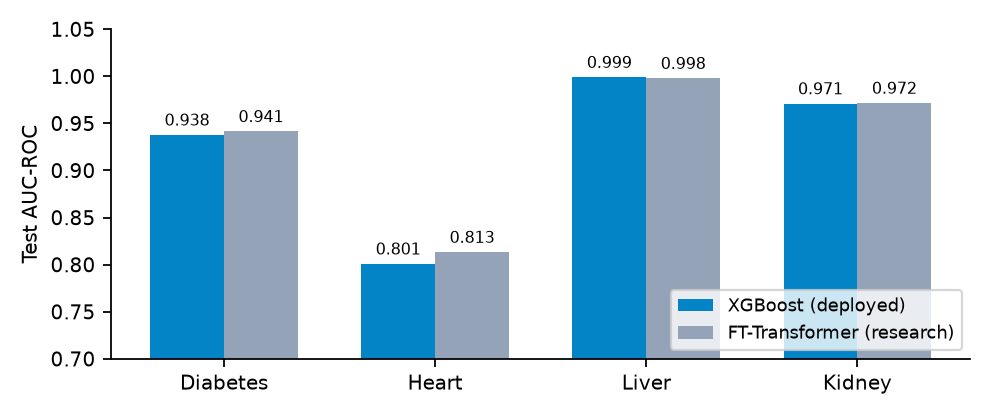
\includegraphics[width=\linewidth]{report_figures/xgb_vs_ft_final.png}
\caption{Final test AUC: XGBoost (deployed) vs.\ FT-Transformer (research).}
\label{fig:ftxgb}
\end{figure}

% ══════════════════════════════════════════════════════════════════
\section{Model Selection: Why XGBoost Was Deployed}
The transformer wins the benchmark --- and XGBoost runs the product. The decision weighed four criteria beyond AUC:
\begin{enumerate}
    \item \textbf{Consistency across tasks:} XGBoost is within $\approx$0.013 of the per-disease winner on every task, so a single training, persistence, and explanation stack covers all four diseases --- operationally cleaner than four bespoke models.
    \item \textbf{Exact explainability:} TreeSHAP gives provably exact per-instance Shapley values for tree ensembles; transformer attributions would require surrogate methods (attention weights are not Shapley values) that weaken the explainability requirement of Section~II-C.
    \item \textbf{Serving cost:} \texttt{.pkl} artifacts, $<$10\,ms CPU inference, no torch/GPU dependency --- the demo and API run anywhere.
    \item \textbf{Artifact reliability:} FT runs across weeks produced inconsistent artifacts; shipping an unstable model as the production head would be indefensible. The proposal itself scoped deep learning as ``enhancement, not requirement'' --- the FT comparison stands as the DL deliverable and a documented future upgrade path.
\end{enumerate}

% ══════════════════════════════════════════════════════════════════
\section{Production System Architecture (Semester 2)}
\subsection{One engine, three surfaces}
The central Semester-2 artifact is a shared inference engine (\texttt{src/inference/engine.py}) that owns artifact loading, patient-vector construction under the sentinel encoding, per-disease prediction, marker-panel readiness/coverage, TreeSHAP contributions, and structured factor formatting. Every user-facing surface calls this engine --- the Streamlit app, the FastAPI service, and the PDF generator --- so predictions are guaranteed identical across surfaces (verified to $10^{-6}$). Fig.~\ref{fig:arch} shows the architecture.

\begin{figure}[t]
\centering
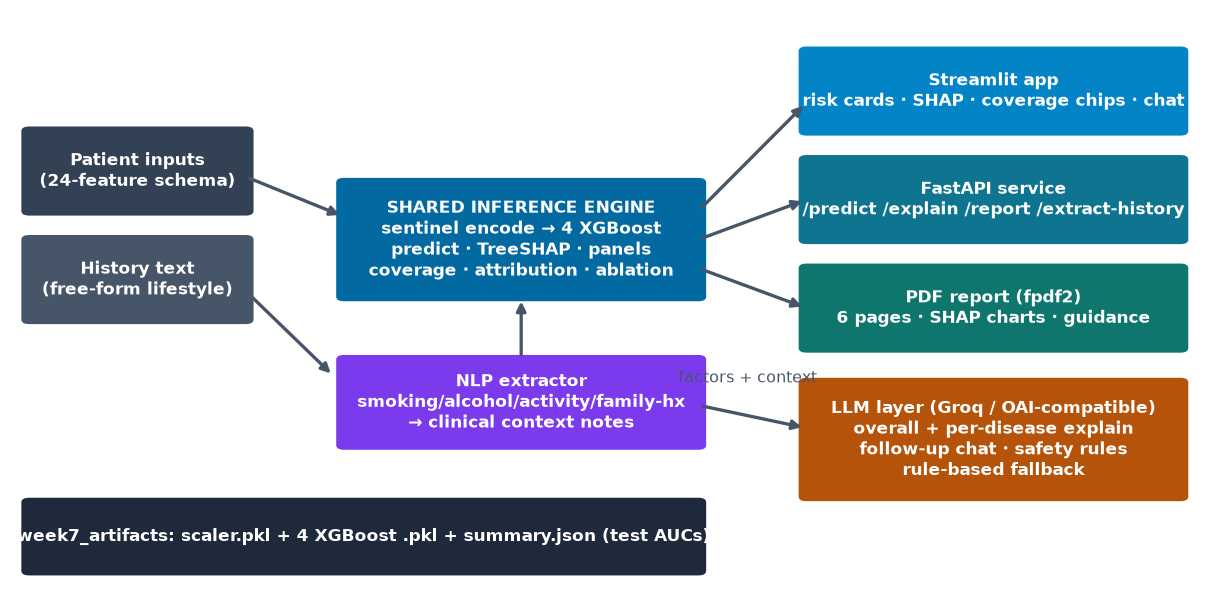
\includegraphics[width=\linewidth]{report_figures/sem2_architecture.png}
\caption{Semester-2 architecture: shared inference engine feeding Streamlit, FastAPI, and PDF; NLP extracts lifestyle context for explanations; the LLM layer consumes structured factors and patient-reported context.}
\label{fig:arch}
\end{figure}

\subsection{Streamlit application}
\texttt{webapp/app.py} implements the patient flow: lab-panel checkboxes (unknown values stay absent --- never forced to enter a number), an optional free-text patient-history box, four risk cards with marker-coverage chips ($n/m$ markers and a completeness bar), per-disease SHAP explanation tabs, cross-disease insight cards, the cross-disease signal expander (attribution + ablation), global feature importance, a PDF download, and the AI explanation/chat section. A sidebar panel surfaces per-disease test AUCs for transparency.

\subsection{FastAPI service}
\texttt{api/main.py} exposes the engine over HTTP with Pydantic request validation and generated OpenAPI docs at \texttt{/docs}: \texttt{GET /health}, \texttt{GET /features} (schema with labels and clinical ranges), \texttt{POST /predict} (all four risks + per-disease coverage metadata), \texttt{POST /explain} (SHAP factors + confidence notes), \texttt{POST /report} (PDF bytes, \texttt{application/pdf}), and \texttt{POST /extract-history} (NLP output). Measured \texttt{/predict} latency is $\approx$7\,ms against the 500\,ms proposal target.

\subsection{PDF patient report}
\texttt{src/report/pdf\_report.py} (fpdf2) generates a six-page report in $\approx$1\,s: a summary page (patient info, provided/missing features, lifestyle table, four-disease risk table with cross-disease footnotes); one page per disease (risk gauge, SHAP driver chart, increasing/decreasing factors, specialist to consult, follow-up tests, diet/lifestyle guidance, red flags, and an amber confidence box when the panel was absent); and a methodology/disclaimer page (Fig.~\ref{fig:pdf}). Because it renders engine output rather than re-implementing prediction, the PDF can never disagree with the app.

\begin{figure}[t]
\centering
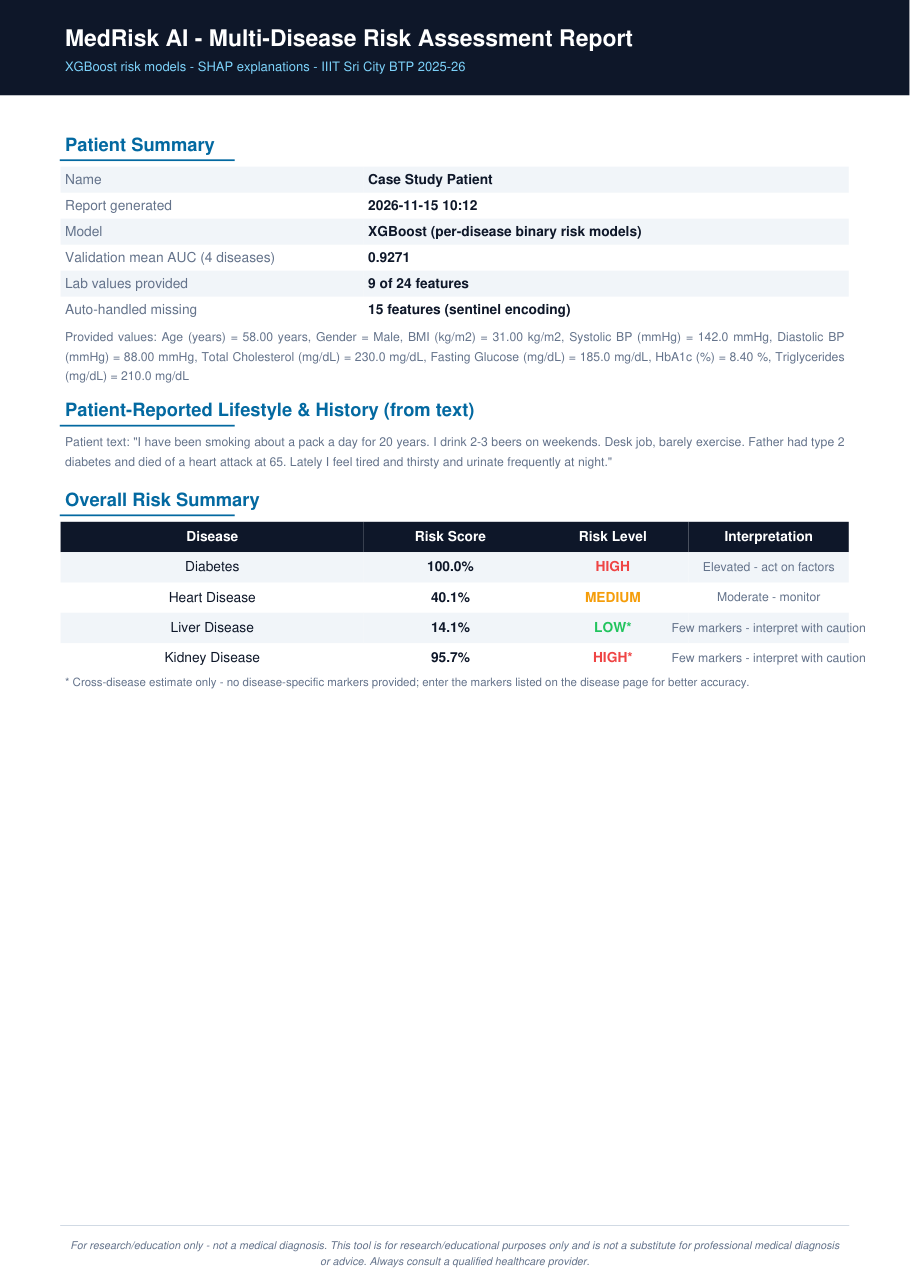
\includegraphics[width=0.9\linewidth]{report_figures/pdf_summary_page.png}
\caption{Generated PDF report --- summary page (real output).}
\label{fig:pdf}
\end{figure}

% ══════════════════════════════════════════════════════════════════
\section{Explainability Layer}
\subsection{Local vs.\ global explanations}
Global importance answers ``what does the model care about overall?'' --- the mean $|$\text{SHAP}$|$ across a reference sample (Fig.~\ref{fig:shap}). Local attribution answers ``why \emph{this} patient, \emph{this} number?'' --- a signed per-feature contribution for one input. Clinical use needs the second: a clinician must see that \emph{this} patient's high score comes from \emph{their} HbA1c, not from a generic importance chart.

\subsection{How TreeSHAP works here}
For each patient vector, XGBoost's \texttt{pred\_contribs} computes exact Shapley contributions $\phi_j$ in log-odds space with the additivity property
\begin{equation}
\mathrm{logit}(\hat{p}) \;=\; \phi_0 \;+\; \textstyle\sum_j \phi_j,
\end{equation}
where $\phi_0$ is the model's base value (the prior logit). Contributions are rendered as diverging bars (red $=$ raises risk, green $=$ lowers), formatted into factor lists (feature, raw value, normal-range status, impact share), and fed to the LLM payload. We verified attributions are genuinely per-instance: for the same model, contribution sums differ by $>$9 log-odds between a diabetic and a healthy profile and the top drivers reorder accordingly (Fig.~\ref{fig:shapcase}) --- the identical $\phi_0$ is the model prior, shared by definition.

\begin{figure}[t]
\centering
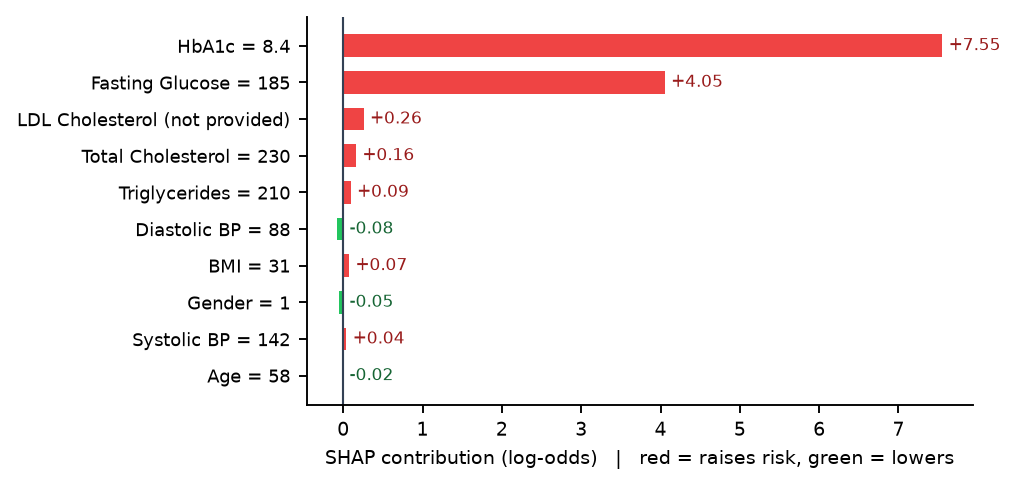
\includegraphics[width=\linewidth]{report_figures/shap_diverging_caseA.png}
\caption{Per-patient SHAP for Case A (diabetes): HbA1c and fasting glucose dominate; signed log-odds contributions.}
\label{fig:shapcase}
\end{figure}

\begin{figure}[t]
\centering
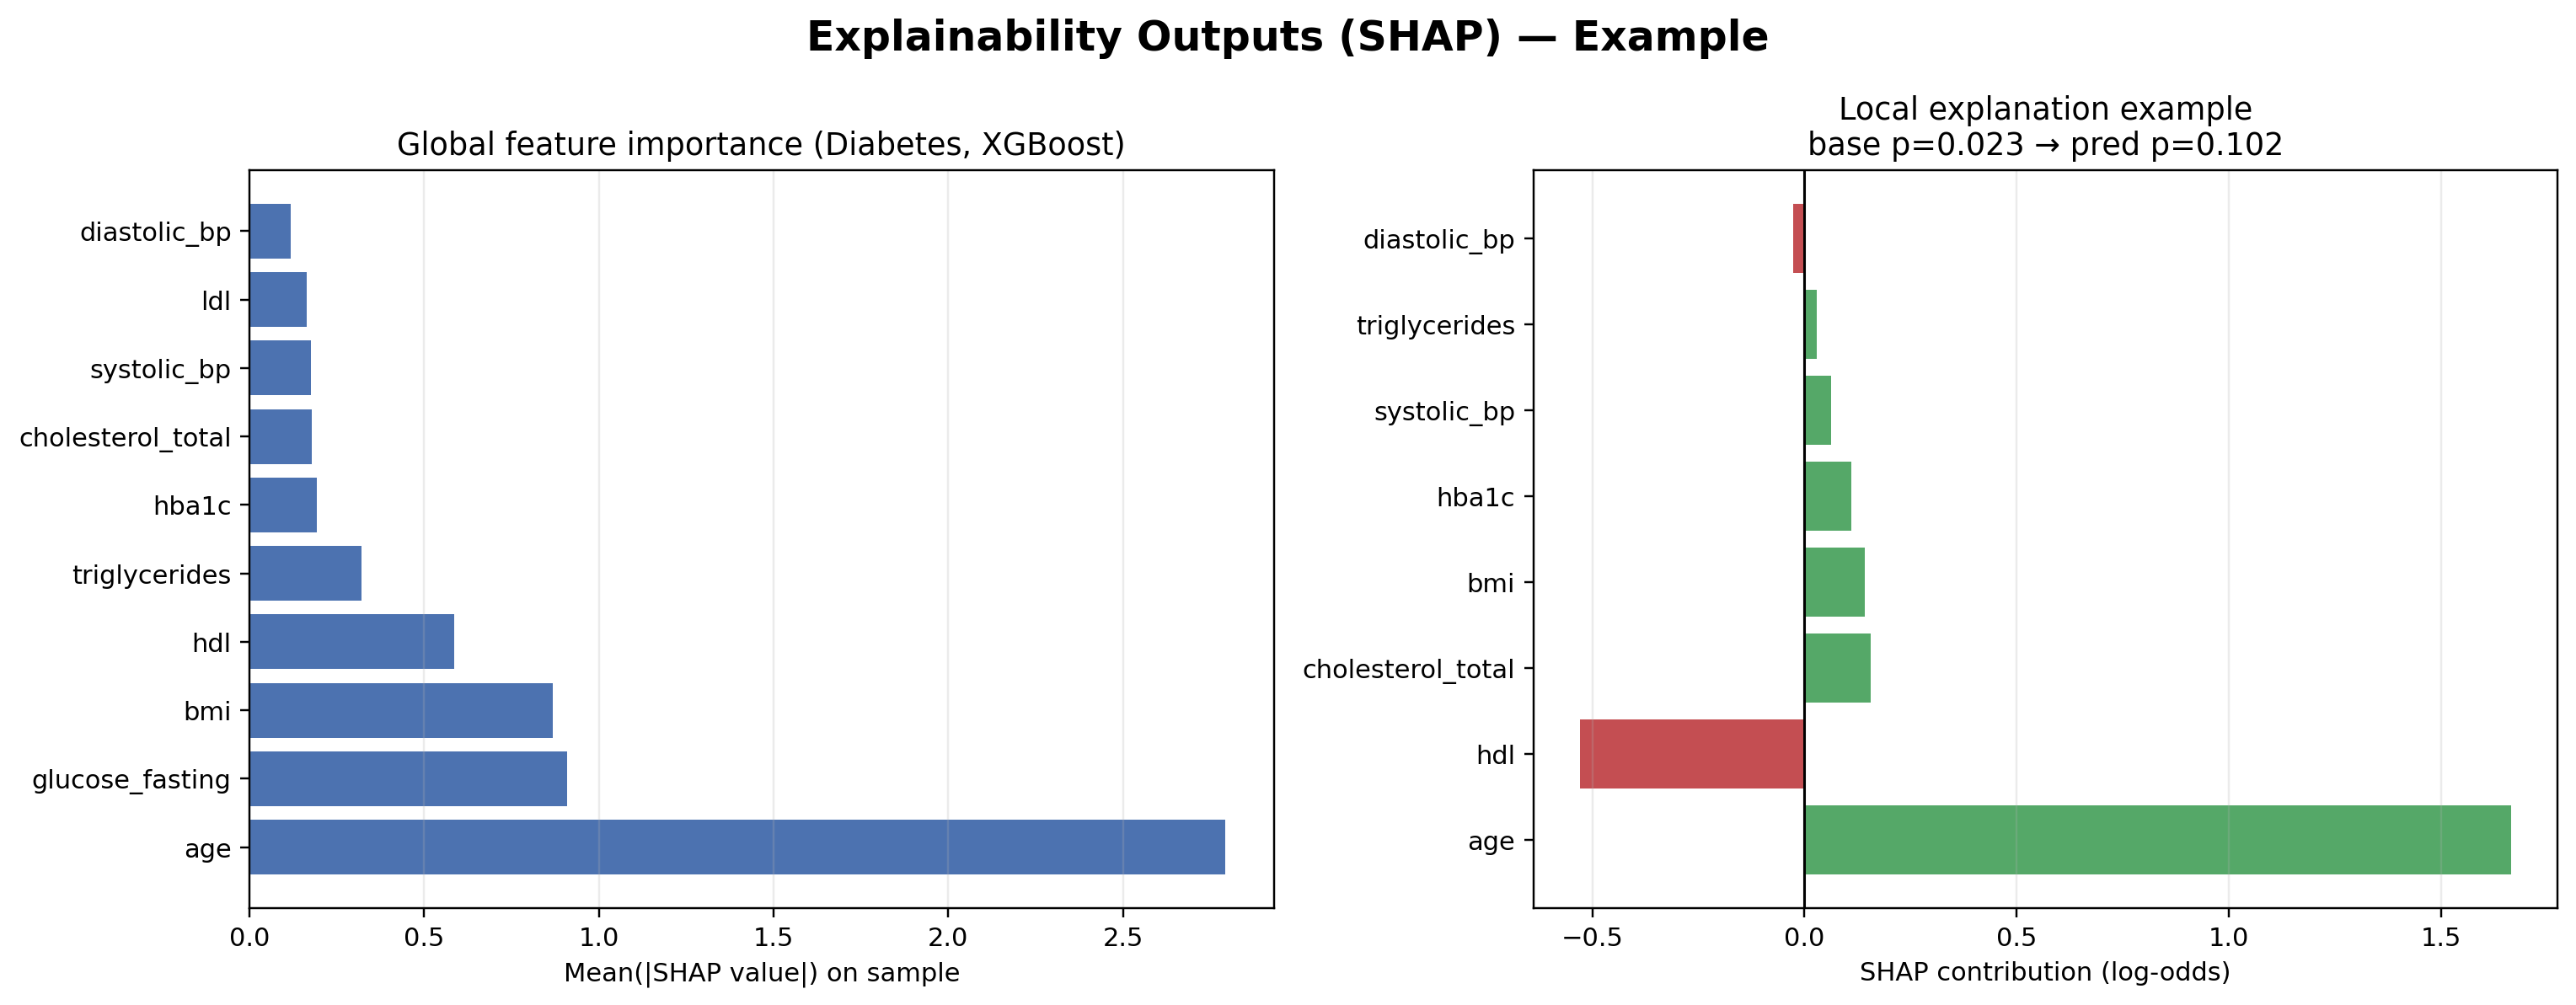
\includegraphics[width=\linewidth]{report_figures/shap_explainability_ui.png}
\caption{SHAP explanations: global importance and per-patient contributions in the UI.}
\label{fig:shap}
\end{figure}

% ══════════════════════════════════════════════════════════════════
\section{Cross-Disease Signal Analysis (Core Contribution)}
Fusion is only a claim until it is measured. Three mechanisms quantify how much one disease's data informs another's score, plus a gate that keeps the claim honest.

\subsection{Patient-level attribution by feature family}
Each disease's per-patient SHAP contributions are summed by \emph{source family} (Demographics, Cardiovascular, Diabetes, Liver, Kidney). For a diabetic patient with \emph{no kidney markers provided}, the kidney score's largest driver is the diabetes family ($+0.63$ log-odds), ahead of cardiovascular ($+0.54$) and demographics ($+0.41$); sentinel-handled kidney features contribute only $+0.41$ (Fig.~\ref{fig:cdattr}). This is the transfer claim made concrete: a disease's risk is measurably driven by another disease's biomarkers.

\begin{figure}[t]
\centering
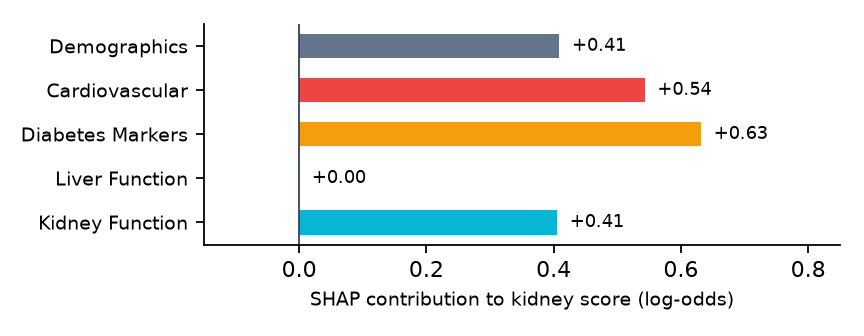
\includegraphics[width=\linewidth]{report_figures/cross_disease_attribution_caseA.png}
\caption{Kidney score attribution by feature family for a marker-less kidney panel (Case A): diabetes markers are the largest single driver.}
\label{fig:cdattr}
\end{figure}

\subsection{Panel ablation}
Each disease is scored three ways --- all features, own-markers-only (demographics + its panel), and markers-removed (Table~\ref{tab:abl}, Fig.~\ref{fig:abl}) --- separating own-panel contribution from cross-disease transfer. The diabetes score collapses 100\%$\to$18.9\% when its panel is removed: it is panel-driven. The kidney score barely moves (96.7\%$\to$95.7\%): for this profile it is cross-disease-driven --- corroborating the attribution result independently.

\begin{table}[t]
\centering
\caption{Panel Ablation --- Case A (risk \%)}
\label{tab:abl}
\small
\begin{tabular}{lccc}
\toprule
\textbf{Disease} & \textbf{All} & \textbf{Own only} & \textbf{Removed} \\
\midrule
Diabetes & 100.0 & 100.0 & 18.9 \\
Heart    & 59.1  & 53.2  & 40.1 \\
Liver    & 11.9  & 15.6  & 11.9 \\
Kidney   & 96.7  & 98.6  & 95.7 \\
\bottomrule
\end{tabular}
\end{table}

\begin{figure}[t]
\centering
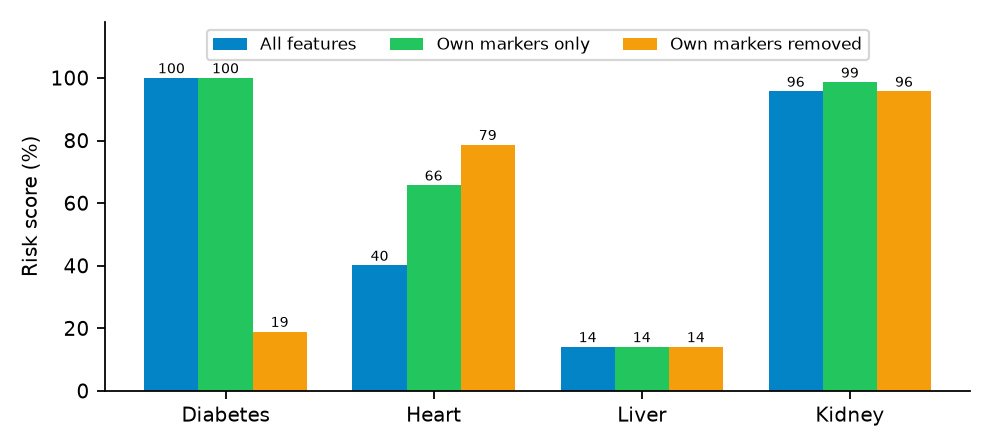
\includegraphics[width=\linewidth]{report_figures/panel_ablation_caseA.png}
\caption{Panel ablation for Case A: full input vs.\ own markers only vs.\ markers removed.}
\label{fig:abl}
\end{figure}

\subsection{Dataset-level interrelation stress test}
At cohort level, each disease was scored using only another disease's source features; transfer is confirmed when the cross-disease signal exceeds a threshold (\texttt{interrelation\_stress\_test.csv}). Result: \textbf{3 of 5 pairs confirmed} --- Kidney$\to$Heart $+0.122$, Liver$\to$Diabetes $+0.131$, Liver$\to$Heart $+0.289$ --- while Diabetes$\to$Kidney ($-0.061$) and Diabetes$\to$Heart ($-0.021$) were not detected at dataset level (Fig.~\ref{fig:stress}). We report the negatives: transfer is real but not universal, which is itself the finding.

\begin{figure}[t]
\centering
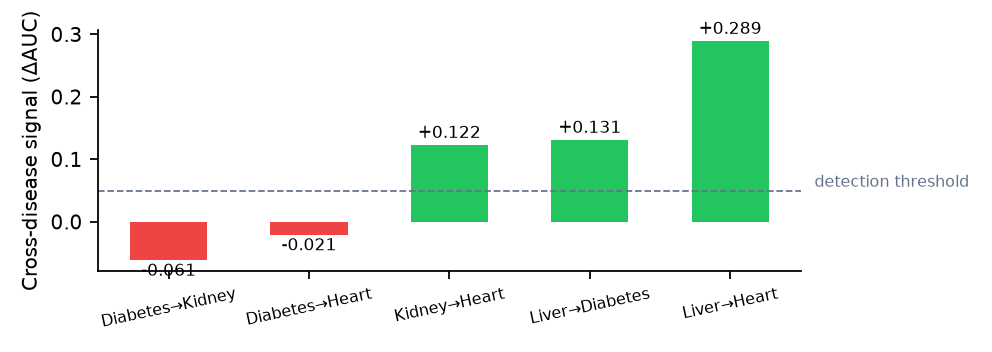
\includegraphics[width=\linewidth]{report_figures/interrelation_stress_test.png}
\caption{Interrelation stress test: cross-disease signal ($\Delta$AUC) per scenario pair; dashed line marks the detection threshold.}
\label{fig:stress}
\end{figure}

\subsection{Marker-coverage gating}
Every disease has a defined own-panel (Diabetes: fasting glucose, HbA1c; Heart: BP + lipid panel; Liver: 8-marker panel; Kidney: creatinine, BUN, GFR, urine protein, hemoglobin). Each card shows $n/m$ markers with a completeness bar, and when zero own-panel markers exist the score is still shown --- hiding it would defeat the fusion purpose --- but flagged ``cross-disease estimate only'' alongside the exact markers that would improve accuracy. This distinction between \emph{cohort-structural} missingness (training-time, handled by encodings) and \emph{patient-side} missingness (inference-time, handled by gating) was motivated by a real testing discovery: the kidney model, trained on $\approx$2{,}032 renal rows, extrapolates to $\approx$95\% risk on empty input because it never saw $-999$ sentinels during training --- an out-of-distribution artifact we chose to surface rather than conceal.

% ══════════════════════════════════════════════════════════════════
\section{NLP Layer}
Patients describe risk factors in prose, not lab panels. \texttt{src/nlp/clinical\_text\_extractor.py} parses free-text history into structured lifestyle factors --- smoking status and amount, alcohol status and amount, physical activity, family history, symptoms, comorbidities, medications --- via ordered regular-expression rules. Two correctness details mattered in practice:
\begin{enumerate}
    \item \textbf{Precedence:} negation/status patterns are evaluated before affirmative ones, so ``I quit smoking 5 years ago'' yields \emph{former}, not \emph{current}; ``drinks daily, heavily'' yields \emph{heavy}, not \emph{unknown}. (A bug here was caught by our own phrase battery and fixed.)
    \item \textbf{Word boundaries:} matching uses whole words, so ``low-salt diet'' cannot trigger the ALT marker and ``in the past'' cannot trigger AST.
\end{enumerate}
Extracted factors surface as UI chips, feed the LLM payload, and populate the PDF history block. A separate patient-facing layer (\texttt{clinical\_context\_notes}) maps factors to plain-language guidance --- ``smoking damages blood vessels and raises heart and kidney risk'' --- deliberately without model jargon. A strict scope boundary holds: \textbf{NLP output enriches explanations; it never alters the 24 structured model inputs} (Fig.~\ref{fig:nlp}). Extraction passed 10/10 phrasing cases; a PubMedBERT hook exists as the upgrade path (Section~XVIII).

\begin{figure}[t]
\centering
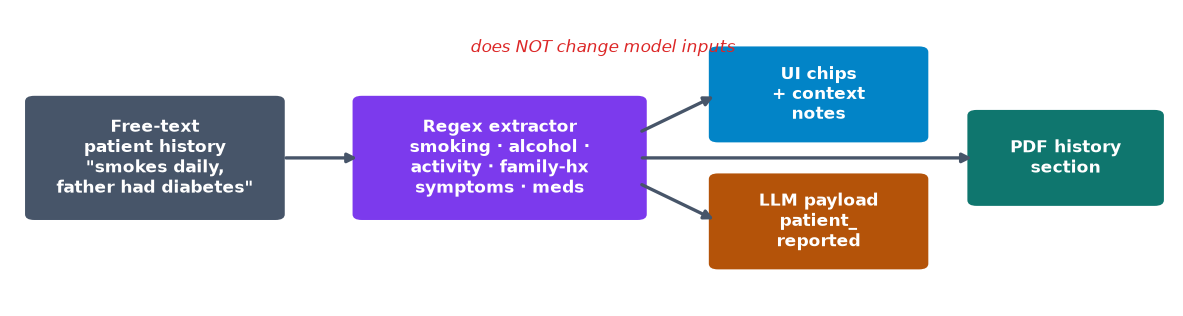
\includegraphics[width=\linewidth]{report_figures/nlp_pipeline.png}
\caption{NLP layer: free text $\to$ structured lifestyle factors $\to$ UI chips, LLM context, PDF history. Model inputs are untouched.}
\label{fig:nlp}
\end{figure}

% ══════════════════════════════════════════════════════════════════
\section{LLM Explanation Layer}
A provider-agnostic OpenAI-compatible client (\texttt{src/llm/}) generates patient-friendly explanations; any compatible endpoint can serve it via environment configuration, and a deterministic rules-based fallback produces identically shaped output when no key or network is available --- the app never dead-ends on an external dependency.

Two scopes exist. \emph{Overall assessment} merges all four disease results into one payload --- ranked risks, per-disease drivers, unified guidance --- so the model reasons over the whole profile rather than one score. \emph{Single-disease} mode explains one result. Follow-up \textbf{chat} keeps the last eight messages as context and routes by word-boundary disease detection with \emph{sticky} targeting: a follow-up like ``any medicines?'' stays on the current disease instead of falling back to generic output (a routing bug where ``salt'' hijacked the liver context was found and fixed via word-boundary matching).

Safety is enforced in the system prompt: no diagnosis, no prescriptions or dosages --- medication classes may only be framed as clinician discussion topics. This is deliberate design: during testing, the model correctly refused ``suggest me medicines so that there is no need to go to doctor,'' redirecting to clinician-guided options --- the behavior a responsible system should exhibit. Responses arrive as structured JSON (summary, factors, next steps, red flags, disclaimer), verified live at $\approx$1\,s latency.

% ══════════════════════════════════════════════════════════════════
\section{Testing and Verification}
The system was verified end-to-end rather than demo-only:
\begin{itemize}
    \item \textbf{Automated suite:} 19 pytest cases covering the engine, readiness/coverage logic, attribution and ablation helpers, NLP extraction, PDF byte generation, and every API route --- all green.
    \item \textbf{Engine battery:} 10 edge-case profiles (empty input, demographics-only, single-marker, extreme high/low values, zeros, negatives) --- all probabilities bounded in $[0,1]$, readiness flags tracking provided panels exactly.
    \item \textbf{Clinical sanity:} ALT-only input $\to$ liver MEDIUM; BP-only $\to$ heart HIGH; creatinine~2.9 $\to$ kidney HIGH; supranormal GFR~200 $\to$ kidney LOW.
    \item \textbf{UI-driven verification:} controls exercised programmatically through Streamlit; rendered output matches engine numbers, and \emph{zero} cross-disease captions appear when all panels are provided (the flag logic correctly goes silent).
    \item \textbf{API/engine parity:} \texttt{/predict} output equals engine output to $10^{-6}$.
    \item \textbf{LLM live verification:} real structured-JSON explanation in $\approx$1.0\,s; chat honors conversation history.
    \item \textbf{SHAP per-patient proof:} contribution sums and driver ordering differ across contrasting patients, refuting the ``same chart for everyone'' concern.
\end{itemize}

% ══════════════════════════════════════════════════════════════════
\section{Proposal Deviations and Justifications}
\begin{itemize}
    \item \textbf{Breast cancer $\to$ kidney disease} (Section~III-B): imaging morphology cannot fuse with a biomarker schema; kidney preserves the fusion thesis and adds the cardiorenal narrative.
    \item \textbf{BioMistral/PubMedBERT $\to$ ordered-regex extractor:} a 7B clinical LLM is disproportionate for short patient-typed histories; the extractor covers the required factors at zero latency and cost (10/10 phrase tests). PubMedBERT remains the documented upgrade path.
    \item \textbf{MIMIC-III notes not used:} credentialing exceeded the semester timeline --- anticipated in the proposal's risk table. Patient-typed history text replaced clinical notes without changing the NLP design.
    \item \textbf{FT-Transformer experimental, XGBoost deployed} (Section~X): reliability and exact explainability outweighed a marginal AUC gain.
    \item \textbf{Cloud deployment, RAG, multi-agent orchestration deferred:} Semester-2 scope was narrowed to what validates the thesis --- fusion quality, cross-disease signal, explanations, and a production-ready local stack.
\end{itemize}

% ══════════════════════════════════════════════════════════════════
\section{Limitations}
\begin{enumerate}
    \item Heart-disease AUC (0.801) is below the 0.85 target --- the weakest label set and lowest schema coverage (29.2\%); richer features (ECG-derived, troponin) would be needed.
    \item Marker-less estimates mix genuine cross-disease signal with sentinel extrapolation; the coverage flag surfaces this honestly, but the residual artifact remains.
    \item The kidney cohort is small ($\approx$2K rows after SMOTE), which partly explains its sentinel-extrapolation behavior.
    \item Models are not clinically calibrated or externally validated; outputs are research estimates, not diagnoses.
    \item The LLM layer depends on an external provider and varies in phrasing; the rule-based fallback covers availability but not phrasing quality.
\end{enumerate}

% ══════════════════════════════════════════════════════════════════
\section{Future Work}
Missingness-aware retraining with random panel dropout (so sentinel inputs become in-distribution, removing the extrapolation artifact at its root); probability calibration and uncertainty estimates; fairness audit across demographics; PubMedBERT/LLM-based history extraction; RAG over clinical guidelines for cited recommendations; multi-agent orchestration; and cloud deployment with monitoring.

% ══════════════════════════════════════════════════════════════════
\section{Conclusion}
This project delivered, end to end, a multi-disease risk prediction platform built on a defensible answer to a real data problem. Four heterogeneous cohorts were fused into one 24-feature schema with missingness treated as information rather than erased; five model families were benchmarked under two encodings with a falsified-and-confirmed hypothesis guiding the choice; XGBoost was deployed for consistency, exact explainability, and serving cost; and a shared engine now serves a Streamlit app, a production FastAPI, and a generated six-page patient report. The second semester added what makes the system trustworthy: exact per-patient SHAP, NLP-extracted lifestyle context, a guardrailed LLM guidance layer, and --- most importantly --- the attribution, ablation, coverage, and stress-test machinery that turns ``one disease's data informs another's risk'' from an assumption into a measured, honestly-bounded result.

\begin{thebibliography}{99}
\bibitem{chen2016xgboost}
T.~Chen and C.~Guestrin, ``XGBoost: A scalable tree boosting system,'' in \emph{Proc. ACM SIGKDD}, 2016.

\bibitem{ke2017lightgbm}
G.~Ke \emph{et al.}, ``LightGBM: A highly efficient gradient boosting decision tree,'' in \emph{Proc. NeurIPS}, 2017.

\bibitem{lundberg2017shap}
S.~M. Lundberg and S.-I. Lee, ``A unified approach to interpreting model predictions,'' in \emph{Proc. NeurIPS}, 2017.

\bibitem{lundberg2020treeshap}
S.~M. Lundberg \emph{et al.}, ``From local explanations to global understanding with explainable AI for trees,'' \emph{Nature Machine Intelligence}, 2020.

\bibitem{gorishniy2021revisiting}
Y.~Gorishniy, I.~Rubachev, V.~Khrapov, and A.~Babenko, ``Revisiting deep learning models for tabular data,'' in \emph{Proc. NeurIPS}, 2021.

\bibitem{chawla2002smote}
N.~V. Chawla, K.~W. Bowyer, L.~O. Hall, and W.~P. Kegelmeyer, ``SMOTE: Synthetic minority over-sampling technique,'' \emph{Journal of AI Research}, 2002.

\bibitem{johnson2016mimic}
A.~E. W. Johnson \emph{et al.}, ``MIMIC-III, a freely accessible critical care database,'' \emph{Scientific Data}, 2016.
\end{thebibliography}

\end{document}
